\newpage
\section{Aufbau}

\begin{figure}[H]
    \centering
    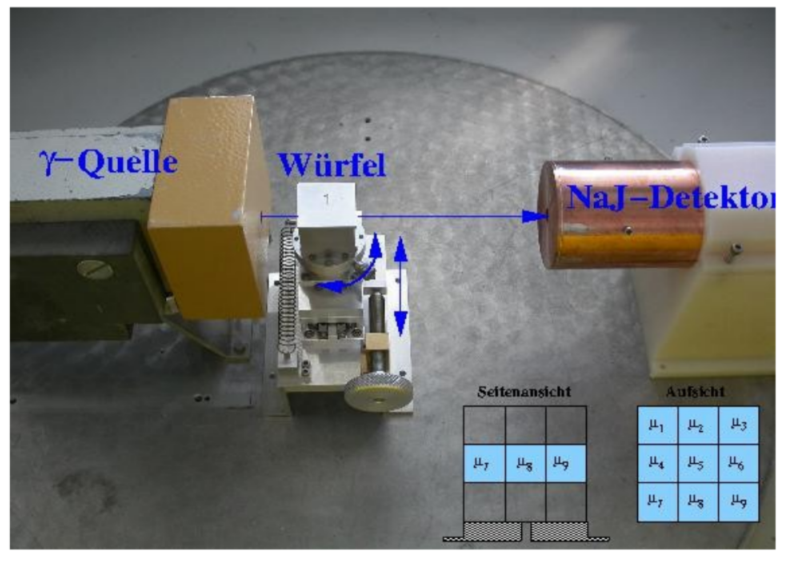
\includegraphics[width=0.55\textwidth]{latex/images/aufbau.PNG}
    \caption{Der Aufbau des \protect \cite{V14}.}
    \label{img:aufb}
\end{figure}

Der Versuchsaufbau, welcher in Abbildung \ref{img:aufb} zu sehen ist, besteht aus einer Cäsium-Probe als $\gamma$-Strahler, 
einem Probenwürfel der auf einer rotier- und verschiebbaren Plattform befestigt ist, und einem $\ce{NaI}$-Szintillationszähler.\\
Die Probe wird dabei von Bleiblöcken abgeschirmt, so dass sie effektiv nur in Richtung des Probenwürfels strahlt. 
Im Strahlengang hinter dem Würfel befindet sich der Szintillationszähler um die Strahlung zu detektieren. 
Dies geschieht über Exzitonen, die in dem Material, durch die Strahlung angeregt werden und beim Zerfall wieder Photonen emitieren. 
Diese werden dann von einem Photodetektor gemessen. Dafür muss der Szintillator aber transparent für seine eigenen erzeugten Wellenlängen sein.\\
Hinter den Detektor ist noch ein Diskriminator geschaltet, welcher Impulse unter einer bestimmten Grenze blockiert, um so den Untergrund herauszufiltern.
Dieser leitet das Messsignal an einen Multichannelanalyzer weiter, welcher die Zählraten abhängig von den korrespondierenden Photonenergien histogrammiert, 
was sich dann über einen Computer ausgeben lässt.

\section{Projektionen}

\noindent
Um über die Gleichung \ref{eqn:mu} die Absorptionskoeffizienten bestimmen zu können muss die Matrix $A$ definiert werden, 
welche für unterschiedliche  Projektionen die korrespondierenden Schichtdicken zu den Absorptionskoeffizienten angibt. 
Die unterschiedlichen genutzten Projektionen sind in Abbildung \ref{img:proj} dargestellt.

%\begin{figure}[H]
%    \centering
%    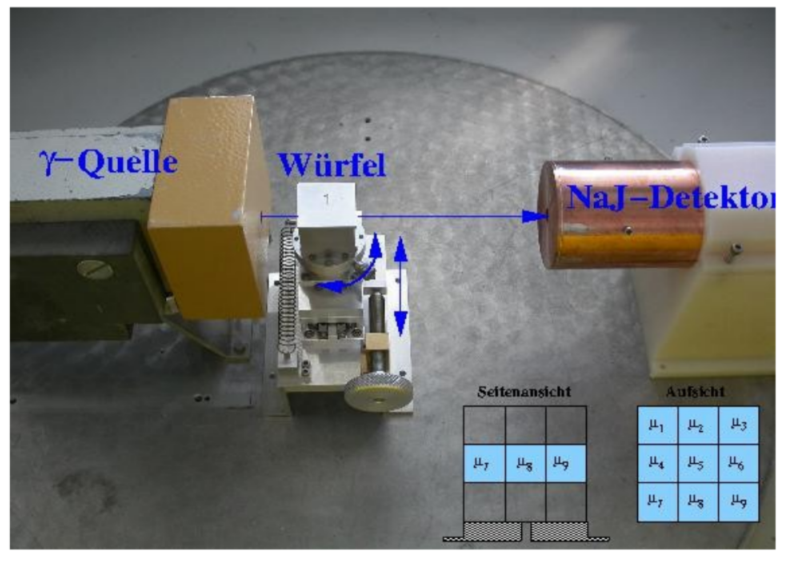
\includegraphics[width=0.7\textwidth]{latex/images/aufbau.PNG}
%    \caption{Der Aufbau des \protect \cite{V14}.}
%    \label{img:aufb}
%\end{figure}

\noindent 
Nach Abbildung \ref{img:proj} ergibt sich beispielsweise für die Projektionen $I_7$ nach Gleichung \ref{eqn:ln}, für die siebte Komponente der Matrix $A$ 
\begin{equation*}
    \ln \left(\frac{I_0}{I_7}\right) = \mu_1 \cdot \sqrt{2}d + \mu_5 \cdot \sqrt{2}d +\mu_9 \cdot \sqrt{2}d \quad .
\end{equation*} 
Dies aufgestellt für alle Projektionen und in Matrixform gebracht führt für die Distanzen zu der Matrix




\begin{equation}
    A \vec \mu = d 
    \begin{pmatrix} 
        1       & 1        & 1      & 0         & 0         & 0         & 0         & 0         & 0         \\
        0       & 0        & 0      & 1         & 1         & 1         & 0         & 0         & 0         \\
        0       & 0        & 0      & 0         & 0         & 0         & 1         & 1         & 1         \\
        1       & 0        & 0      & 1         & 0         & 0         & 1         & 0         & 0         \\
        0       & 1        & 0      & 0         & 1         & 0         & 0         & 1         & 0         \\
        0       & 0        & 1      & 0         & 0         & 1         & 0         & 0         & 1         \\
        \sqrt{2}& 0        & 0      & 0         & \sqrt{2}  & 0         & 0         & 0         & \sqrt{2}  \\
        0       & 0        &\sqrt{2}& 0         &\sqrt{2}   & 0         &\sqrt{2}   & 0         & 0         \\
        0       & \sqrt{2} & 0      & 0         & 0         & \sqrt{2}  & 0         & 0         & 0         \\
        0       & 0        & 0      & \sqrt{2}  & 0         & 0         & 0         & \sqrt{2}  & 0         \\
        0       & \sqrt{2} & 0      & \sqrt{2}  & 0         & 0         & 0         & 0         & 0         \\
        0       & 0        & 0      & 0         & 0         &\sqrt{2}   & 0         & \sqrt{2}  & 0         \\
    \end{pmatrix} \cdot
    \begin{pmatrix} 
        \mu_1  \\
        \mu_2  \\
        \mu_3  \\
        \mu_4  \\
        \mu_5  \\
        \mu_6  \\
        \mu_7  \\
        \mu_8  \\
        \mu_9  \\
    \end{pmatrix} \quad.
    \label{eqn:A}
\end{equation}

		
\section{Durchführung}

\noindent 
Zuerst wird der $\ce{^{137}Cs}$-Strahler wird in einer Bleihalterung befestigt.
Während keine Probe sich im Strahlengang befindet wird die Grundintensität $I_0$ gemessen.
Dafür wird auf dem Computer im Programm MAESTRO eine Messdauer von $\SI{240}{\second}$ eingestellt.
Aus den Ergebnissen lässt sich dann die Höhe und Halbwertsbreite des Photopeaks ablesen.\\
Anschließend wird eine Messreihe mit dem Würfel 1 durchgeführt. Dieser besteht nur aus dem Aluminiumgehäuse, welches die anderen Würfel umgibt.
Dafür wird der Würfel im Strahlengang platziert und für drei Projektionen die damit korrespondierenden Spektren aufgenommen.\\
Dieses Vorgehen wird für die Würfel 2 und 3, welche aus reinen Materialien bestehen, wiederholt. 
Die möglichen Materialien sind dabei Aluminium, Messing, Delrin, Blei und Eisen.\\
Der Würfel 4 besteht aus neun kleineren Elementarwürfeln, welche auch aus diesen Materialien bestehen.
Dieser wird zuletzt in den Strahlengang gesetzt und dort die mittlere Ebene für alle zwölf möglichen Projektionen ausgemessen.